\chapter{Fixing Datasets: \acsp{GAN} \& \acsp{VAE}}

Deep Learning has proven to be successful at generating natural images. \citet{dagan} see in this ability an opportunity to improve datasets by generating more data and shows performance improvements in classifiers when using generated data as a supplement to the training data.

Using generative models in the context of face recognition is appealing. Many pictures per identities are needed in order to teach a classifier that it should be invariant to lighting, pose, makeup, haircuts, etc. However, as we grow the number of identities that the system has to recognize, there is a risk that the classifier does not learn the invariants for identities with less variations in training data. In other words, we fear that the classifier learns useful features only for the identities with many diverse pictures and overfit the case with little training data.

Generating data gives us the opportunity to create the diversity of pose, lightning etc for the identities with the least diverse identities.

In this chapter we lay out a review of the different techniques of generative models we explored before settling on one. We then introduce our chosen system for data augmentation in the context of face recognition.

\section{Generative models for building invariances}

In our dataset, some people were always facing the camera, or never smiling, while others exhibited larger variations in pose, exposition or image quality. We hypothesized that this could lead the classifier to learn some shortcuts like "This is not Person \textbf{A} because that person is smiling, \textbf{A} never does". One obvious way to teach invariance to classifier is to feed them proper data exhibiting those invariances. In face recognition, that would translate in making sure that all identities have various level of illuminations and a wide variety of poses so that the classifier does not learn shortcuts. We aim to complement the dataset with the missing variations of each identity by training a generative model. Hopefully, the model would learn the general concepts of face geometry, disentangle it from facial identity, and could reenact anyone's face into any pose.

\section{Problem definition}

Let $\mathcal{D}$ be a dataset containing some face pictures $x_i$ and their identity label $y_i$ such that $(x_i, y_i) \in\mathcal{D}$. Let $p_i \in \mathcal{P}$ be an unknown semantic latent vector representing pose, lighting etc, containing no information about $y_i$, such that a powerful generative model $G$ could hold $G(y_i, p_i) = x_i$ (see figure \ref{fig:G_specs}).

Those faces can be considered samples of an underlying "face photo" manifold with dimensions describing semantic variations such a lighting, pose or identity. We would like to learn a generator $G(y_i, z), z \sim p_Z(z)$. $G$ learns to interpret $z$ as a $p_i$ and decode it as a pose / illumination / etc vector that doesn't include any identity information. Ideally, $z$ is a probability distribution that is easy to sample from (eg standard normal). We could then reenact any identity $y$ by sampling $z$ vectors at will.

\begin{figure}[ht]
    \centering
    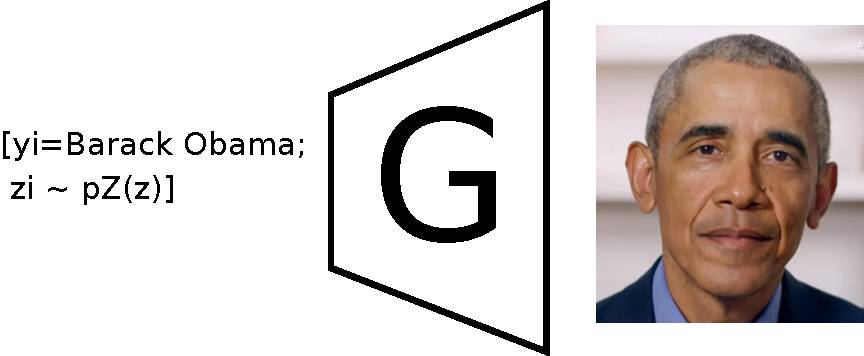
\includegraphics[scale=0.5]{60-files/GANVAE-1-1}
    \caption{$G$ is a generator that turns a person identitifier $y_i$ and a latent variable $z_i$ into an image.}
    \label{fig:G_specs}
\end{figure}

\section{Generative Models}
\subsection{Fundamentals}
When trying to generate data, we wish to model $P(X)$ for any data distribution $X$ in terms of its individual components. For instance, for image data, we learn to model images $x \in \mathcal{X}$ by modeling the color probability distribution of each of its pixels $x_{1..H, 1..W}$, by assuming independence.

\begin{equation}
\label{gen_model1}
    P(X=x) = \prod_{i=1}^H \prod_{j=1}^W P(X_{i, j}=x_{i, j})
\end{equation}

With such a simple model, $P(X_{i, j})$ is left as an arbitrarily sophisticated or simple distribution of our choice, such as a categorical distribution over discretized pixels values (with parameters $\theta_{i,j}$)

\begin{equation}
    P(X_{i, j}) = \texttt{Cat}(X_{i,j}; \theta_{i,j})
\end{equation}

or Gaussian distributions over values (with mean parameters $\mu_{i,j}$ and standard deviation parameters $\sigma_{i,j}$)

\begin{equation}
P(X_{i, j}) = \mathcal{N}(X_{i,j}; \mu_{i,j}, \sigma_{i,j})    
\end{equation}


Once the individual pixel probabilities parameters (ie $\theta_{i,j}$ or $\mu_{i,j}, \sigma_{i, j}$) have been estimated from data, one could sample a value for each pixel and get an image.

However, this modeling is trivial and would produce pictures that looks nothing like real images because it considers each pixel as independent and does not take into account patterns and spatial correlations. Deep learning has not come to the rescue... yet.

\subsection{Auto-regressive models}

This components independence assumption leads to very poor results, especially in image generation. Instead of sampling each component independently, we could sample each component one after another, in any predefined order, based on some of the previously sampled values. In which case $P(X_{i,j})$ becomes a distribution conditioned on the previous $k$ components. The graphical model is illustrated in figure \ref{fig:autoreg-chain}.

For image data, those individual components are pixels, and a full image is sampled pixel by pixel. Each sampling operation operates on a context window constituted of the previous samplings. As we consider bigger context windows $k$, the models needed become more complex and bigger and that is when Deep Learning comes into play. This image is progressively sampled following an ordered set of pixel coordinates $\Psi$ (usually left to right and top to bottom, but not limited to).

\begin{equation}
    P(X) = \prod_{i = 0}^{|\Psi|} p(X_{\Psi_i} | x_{\Psi_{i-1}}, .., x_{\Psi_{i-k}})
\end{equation}

This is the approach coined by PixelCNN \citep{pixelcnn}, PixelRNN \citep{pixelrnn}, PixelCNN++ \citep{pixelcnn++} or PixelSNAIL \citep{pixelsnail}. At inference time, we sample pixels one by one, each requiring a model forward pass. This exhibits the major drawback of auto-regressive models for image synthesis: they require $H \times W$ forward passes, making it extremely slow and computationally intensive. Moreover, as the images grow bigger, not only more forward passes are needed, bigger models are needed as well in order to grow their receptive fields and context windows accordingly. A single pass of PixelCNN is shown in figure \ref{fig:pixelcnn}.

\begin{figure}[ht]
    \centering
    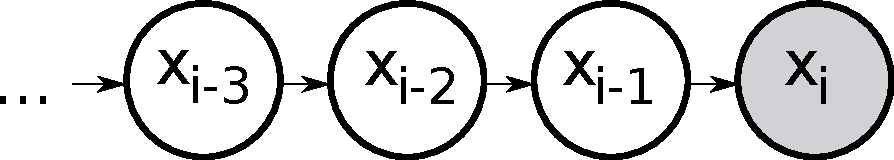
\includegraphics[scale=0.5]{60-files/chain-pixelcnn.pdf}
    \caption{Conditional probability graph of an autoregressive model. Each pixel depends on the previous ones, in an iterative fashion.}
    \label{fig:autoreg-chain}
\end{figure}

\begin{figure}[ht]
    \centering
    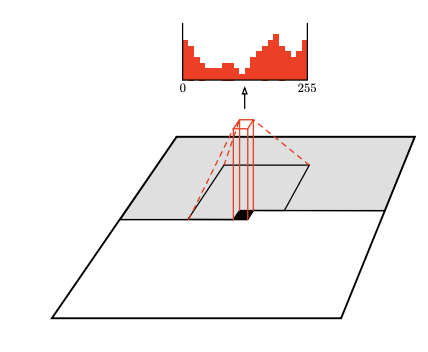
\includegraphics[scale=0.8]{60-files/pixelcnn.png}
    \caption{A PixelCNN sampling a pixel value for the current pixel from its surrounding context. White pixels are still undetermined grey pixels have already been sampled. Shown in red is the softmax output describing the probability distribution of the current pixel values conditioned on the context window. Image from \citet{pixelcnn}}
    \label{fig:pixelcnn}
\end{figure}


Modern auto-regressive models such as the \ac{VQVAE} \citep{vqvae} or \ac{VQGAN} \citep{vqgan} try working around this complexity by only sampling small pictures or small representations, leaving the actual high quality rendering to another method, such as convolutional upsamplers, convolutional decoders, or \acp{GAN}. The \ac{VQVAE} will be described in section \ref{section:vqvae}.

\section{Latent-Variable Models and Variational AutoEncoders}
\subsection{Principles}

\begin{figure}[ht]
    \centering
    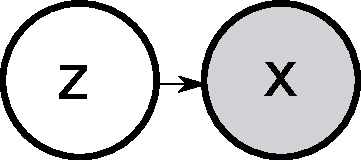
\includegraphics[scale=0.5]{60-files/chain-vae.pdf}
    \caption{Conditional probability graph of a Latent Variable Model (LVM). The whole image $x$ is sampled at once from a lower dimensional encoding $z$.}
    \label{fig:vae-chain}
\end{figure}

Instead of having a long chain of random variable dependency (ie the previous components), we can assume that there is a lower dimensional code $z \sim p(z)$ that explains the data, and that a powerful function could decode from it all the components at once (compare figure \ref{fig:autoreg-chain} and \ref{fig:vae-chain}). For images, this embodies the idea that the pixels of an image can be reduced to a much denser amount of semantic information such as "a child sitting on a bench and eating ice cream in a park" or a low dimensional feature vector. We can thus model the data probability density as the probability of a data point $x$ decoded by all possible codes $z$:

\begin{equation}
    P(X) = \int P(X | z)p(z)dz = \int p(z) \prod_{i=1}^H \prod_{j=1}^W P(X_{i,j} | z) dz
\end{equation}

\begin{equation}
\label{eq:logppx}
    - \log p(X) = - \log \int p(z) P(X | z) dz
\end{equation}

In our case, this code $z$ is considered unknown and has to be discovered by the training procedure as well. We often chose $z$ to be a continuous feature vector and $p(z)$ to be a standard Gaussian as it is easy to sample from. $P(X | z)$, called "decoder", generates the data components from the code. It usually is a neural network suited for the data type.

The integral in Eq \ref{eq:logppx} can be rewritten as an expectation: 

\begin{equation}
    - \log p(X) ~= - \log \IE_{z \sim p_Z(z)}[P(X| z)]
\end{equation}

The expectation outside the $\log$ is unfortunate: the log of the expected value would need many samples in order to be accurate, and all those probability multiplications would be numerically unstable.

Thankfully, Jensen's inequality gives us a useful lower bound: $f(\IE[x]) \leq \IE[f(x)]$ for any convex function $f$. So, the $\log$ can be moved inside the expectation at the cost of a lower bound.

\begin{equation}
    - \log p(X) \leq \IE_{z \sim p_Z(z)} [- \log  P(X | z) ]
\end{equation}

Learning this model with Maximum Likelihood Estimate for large datasets is impractical as we would first need to sample a $z$, find a sample in the dataset that is best explained by the decoder for that $z$, and perform the MLE step.

The VAE \citep{vae} proposes to solve this with more neural networks. The simple fix is to learn an "encoder" $q$ that learns which $z = q(x)$ explains $x$ the best. We can then take a training sample, encode it to a $z$, decode it back, and optimize for reconstruction and penalize the log probability of $z$ according to the prior $p(z)$ as well.

This, however, would not make a good generative model as there is no incentive that the encoder covers the whole volume of $p(z)$. Instead of encoding $z = q(z|x)$ as a deterministic mapping, $q(z|x)$ can be turned into probability density parameters from which we can sample $z$. We can thus read $z \sim q(z|x)$, and instead of penalizing the log probability of $p(Z=z)$, we penalize the $D_{KL}(q(z|x) || p(z))$. With $q$ being pushed to resemble the prior, we hope to enforce full utilization of the prior probability space.

Formally, if we use this surrogate distribution $q(z|x)$ to ease smart sampling from $p(z)$, we are doing \emph{importance sampling}, and get $\IE_{z \sim p(z)} [P(x|z)] = \IE_{z \sim q(z|x)}[\frac{p(z)}{q(z|x)}P(x|z)]$. Taking the log and applying Jensen's inequality, we obtain

\begin{equation}
\begin{split}
    - \log p(X) & = - \log \IE_{z \sim p_Z(z)} [P(X | z) ] \\
    & = - \log \IE_{z \sim q(z|x)} [ P(X | z) \frac{p_Z(z)}{q(z|x)} ] \\
    & \leq \IE_{z \sim q(z|x)} [- \log P(X | z)  - \log \frac{p_Z(z)}{q(z|x)}] \\
    & \leq -\IE_{z \sim q(z|x)}[\log P(X | z)] + \IE_{z \sim q(z|x)} [- \log \frac{p_Z(z)}{q(z|x)}] \\
\end{split}
\end{equation}

This formalizes the \ac{ELBO}:

\begin{equation}
    - \log P(X) \leq ELBO(x) = - \IE_{z \sim q(z | x)} \log p(X | z) - D_{KL}(q(z | x) || p_Z(z))
\end{equation}

We usually interpret this loss as two terms that must be minimized: a reconstruction term and a prior divergence term. While this helps this intuitive explanation is the source of some misconceptions that are beyond the scope of this document.

\subsubsection{The reparameterization trick}

It is important to note that sampling is a discrete operation. As $z$ is sampled from $q$, it is not natural to learn both $q(z|x)$ by backpropagation. In order to be able to backpropagate into $q$ we have to make it a differentiable operation.

In order to do so we model $q$ as an isotropic Gaussian of D dimensions. We make the neural network modeling $q$ output two sets of values: $\boldsymbol{\mu}(z|x)$ and $\boldsymbol{\sigma}(z|x)$, ie the mean and standard deviation of each dimension of the Gaussian. We observe that sampling from $\mathcal{N}(\boldsymbol{\mu}(z|x), \boldsymbol{\sigma}(z|x))$ is the same as sampling from $\boldsymbol{\mu}(z|x) + \boldsymbol{\sigma}(z|x)\mathcal{N}(0, \mathbf{I})$. Elementwise addition and multiplication are differentiable, therefore this form allows to backpropagate into $q$. This is known as the reparameterization trick.


\subsection{Limits}

It is to be noted that the shortcomings of the VAE are well known:

\begin{enumerate}
    \item The KL term and sampling operation prevents the decoder from having an accurate latent variable to decode. Thus, the produced samples are notoriously blurry.
    
    \item The reconstruction term and divergence term balance in counter-intuitive ways. The ultimate VAE goal is not to learn a meaningful latent vector but to assign the correct probability density to the data distribution. When possible, the encoder ignores the input sample, produces exactly the prior distribution (turning the KL term to zero), and decodes samples at random. This is to be expected, especially when powerful decoders are used.
\end{enumerate}



\subsection{Information Bottleneck}

\subsubsection{General concept}

The reparameterization trick and the KL term to fit a noise distribution inspired a variational information bottleneck, as a layer. Through this layer, only the information necessary for minimizing the task's loss would go through in a compressed way. All the unnecessary information would be eliminated to resemble the prior noise distribution.

\subsubsection{Benefits as regularization}

\citet{informationbottleneck} inspects how models with an information bottleneck generalizes. It happens that those models are less prone to overfitting and adversarial attacks, and generalize better overall.

\subsubsection{In Latent Variable Models}
\label{sec:lvm}

\begin{figure}[ht]
    \centering
    \includegraphics[scale=0.75]{60-files/latent-bottleneck.pdf}
    \caption{Training a latent variable model for colorization. There are multiple possible colorizations for a single greyscale input. A latent extractor $h$ extracts the information solving the ambiguity between those multiple answers ; an information bottleneck prevents the latent extractor from encoding all of the target and short-circuiting the task. The colorizer $f$ resolves ambiguous cases using the latent.}
    \label{fig:latent-bottleneck}
\end{figure}

This idea is also useful in latent variable models and multimodal tasks. In image colorization for instance (illustrated in figure \ref{fig:latent-bottleneck}), naive supervised training is unable to represent that many colors might fit an object, and the neural net would produce grey-ish pictures without vibrance, actually outputting the average color of the possible responses.

While \acp{GAN} fit this issue, they come with their own difficulties. Instead, we can still use a Maximum Likelihood Estimate framework by extracting a latent variable from the target. An information bottleneck on that latent variable prevents the target to bleed through and ensure it only contains the information to complete the task that can't be deduced from the input.

At inference time, we can either use latent-variables extracted from predefined samples, sample from the prior noise distribution, or learn a prior from the extracted train latents (such as a Gaussian mixture model).

Designing an efficient information bottleneck is challenging: it must not leak any redundant or useless information, must not filter out the needed information, and it is interesting to be able to sample from it.

\subsection{\ac{VQVAE}}
\label{section:vqvae}

\subsubsection{Architecture}

\begin{figure}[ht]
    \centering
    \includegraphics[scale=0.5]{60-files/vqvae-train-1.pdf}
    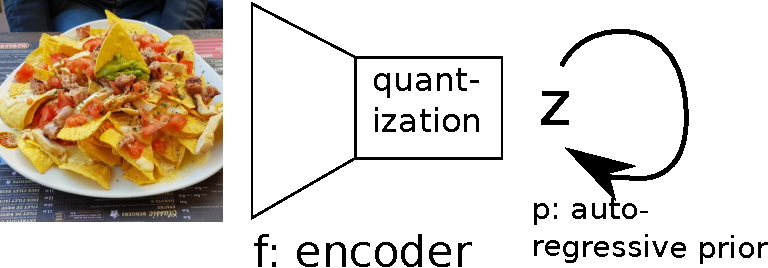
\includegraphics[scale=0.5]{60-files/vqvae-train-2.pdf} \hspace{1cm}
    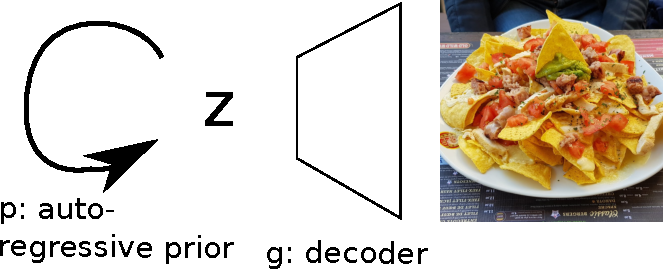
\includegraphics[scale=0.5]{60-files/vqvae-sample.pdf}
    \caption{\textbf{top}: Training a \ac{VQVAE} stage 1: a quantized encoder and decoder are trained in an autoencoding fashion. \textbf{bottom left}: Training a \ac{VQVAE} stage 2: the encoder is frozen and an autoregressive prior is learnt on the extracted latents. \textbf{bottom right}: Sampling from a \ac{VQVAE}: We generate a latent variable from the prior model and decode it to a full picture}
    \label{fig:vqvae-train}
\end{figure}

The \ac{VQVAE} \citep{vqvae} takes the VAE from another perspective. They propose to train an auto-encoder then, in a second stage, fit an auto-regressive model on the latent representation as a prior to sample from. In order to both ease the job of the prior network and control the amount of information that can be transmitted, the latent is encoded as discrete tokens.

For image data, the prior network usually is a PixelCNN or a variation of it. The approach is summed up in figure \ref{fig:vqvae-train}.

\subsubsection{Backpropagating through quantization}

Besides those architectural novelties, the main contribution of the work was to provide a backpropagation-friendly discretization operation.

In order to discretize, the quantization layer $q$ maintains a codebook $c$ of K vectors, K being a hyperparameter. The continuous activation vectors $x$ are replaced by their closest neighbor in the codebook, effectively quantizing with a resolution of K.

\begin{equation}
    q(x, c)=c_i, \text{ where  } i= \argmin_j ||x - c_j||_2
\end{equation}

In the backward pass, the gradient is forwarded both to the prototypes in the codebook and used as an approximate gradient to the pre-quantization activations. In addition, a second loss term, called "commitment loss", with weight $\beta$ encourages the continuous activations and prototypes to remain close under a L2 distance. The commitment helps keeping the gradient forwarded to the activations remaining a meaningful approximation, although computed from their quantized counterparts.

We need to backpropagate the gradient of loss $l$ through this quantization, as well as compute the gradients with respect to the codebook. We use the chain rule, as follows:

\begin{equation}
    \frac{\partial q(x, c)}{\partial c} = \frac{\partial l}{\partial q(x, c)}
\end{equation}

\begin{equation}
\begin{split}
    \frac{\partial q(x, c)}{\partial x} &= \frac{\partial l}{\partial q(x, c)} + \beta \frac{\partial (x - q(x, c))^2}{\partial x} \\
    & = \frac{\partial l}{\partial q(x, c)} + 2\beta x(x - q(x, c)) \\
\end{split}
\end{equation}

\subsubsection{Benefits}

As the latent variables usually have a lower dimensionality than the data points, it is faster to train and sample latents from an autoregressive model, than to train and sample from an autoregressive model on the data points directly.

The generated samples are also of much greater quality that ones of a standard VAE. First, The prior distribution is much more complex, hence much more expressive. Secondly, the component-by-component, conditional, sampling, instead of sampling all the latent at once like a standard VAE allows for a much more precise latent.

\subsubsection{As an information bottleneck}

When designing a quantization layer in a neural network, we can choose how many codebooks and quantized values per codebook we want. This allows to set a very accurate and hard limit on the maximum amount of information that can be transmitted. For instance, with 8 codebooks with 32 codepoints, we can transmit exactly $8 \log 32 = 8 \times 5 = 40$ bits of information.

\section{GAN}
\subsection{Principles}

\begin{figure}[ht]
    \centering
    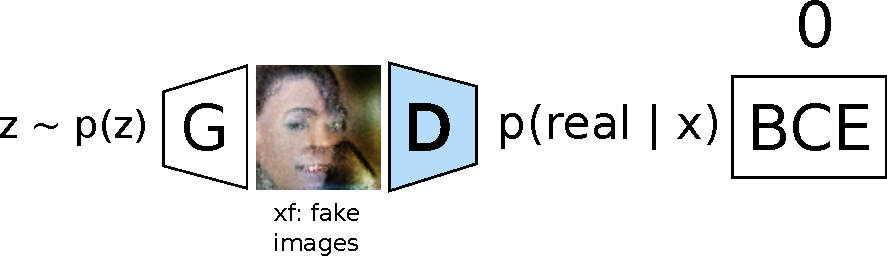
\includegraphics[scale=0.5]{60-files/gan-learn-D-fake.pdf} \hspace{1cm}
    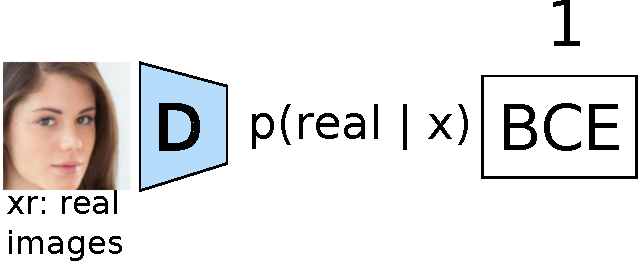
\includegraphics[scale=0.5]{60-files/gan-learn-D-real.pdf}
    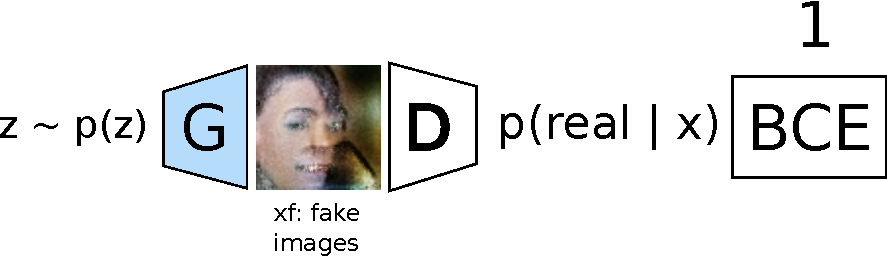
\includegraphics[scale=0.5]{60-files/gan-learn-G.pdf}
    \caption{Training a standard \ac{GAN}. \textbf{top left}: $G$ is kept frozen, we teach $D$ to classify a fake sample as a fake image with a binary cross entropy loss and target 0. \textbf{top right}: $D$ is taught to classify a real sample with BCE target 1. \textbf{bottom}: we train $G$ to produce images that are classified as true by $D$, $D$ is kept frozen.}
    \label{fig:gan-training}
\end{figure}

\subsubsection{\acp{GAN} as competition}


\newcommand{\pdata}[0]{p_\texttt{data}}
\newcommand{\pfake}[0]{p_\texttt{fake}}
\newcommand{\ppath}[0]{p_\texttt{path}}

Another completely different family of generative model are \acp{GAN}. \acp{GAN} do not model $P(X)$ explicitly, neither do they compute the log likelihood, exact or approximated. In the literature, \acp{GAN} are presented as two neural networks competing against each other. A \ac{D} learns to discriminate samples from the real data distribution $\pdata$ and the fake samples from distribution $\pfake$ produced by a \ac{G}. The two networks are trained in an alternating and opposite fashion, $D$ learning to discriminate better while $G$ learns to fool $D$ by gradient ascent. The optimal state is reached when $\pfake = \pdata$.

While a lot of engineering went into designing better $G$s for image synthesis of various kind \cite{progan,stylegan,stylegan2,msggan}, $D$s got most of the theoretical work as they provide the signal $G$ trains against and are the only component in contact of the true data distribution.

Those three training steps are illustrated in figure \ref{fig:gan-training}.

\subsubsection{\acp{GAN} as learnable loss}

\begin{figure}[ht]
    \centering
    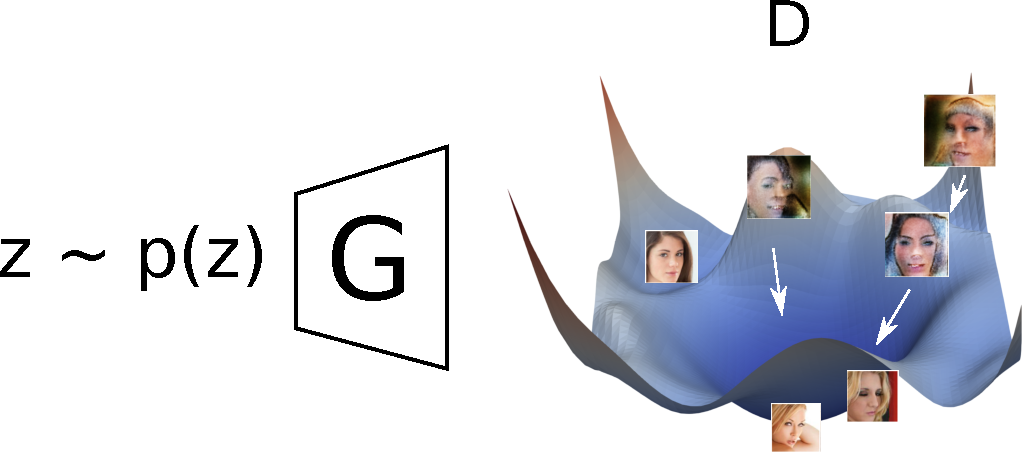
\includegraphics[scale=0.5]{60-files/gan-as-loss.pdf}
    \caption{Interpreting $D$ as a trainable loss giving low values to real samples and high values to fake samples. $G$ learns to minimize the loss $D$ represents. Gradients of fake samples represented as white arrows.}
    \label{fig:gan-training-energy}
\end{figure}

Alternatively, they can be viewed as a simple but rich idea: training a neural network as loss function, modeling the manifold of the data distribution. This loss-neural-network learns to give high logits to samples coming from the real data distribution and low logits to samples produced by a generator network. The generator networks is trained to maximize the discriminator's output, and convergence is reached when it perfectly mimics the data distribution, making a flat logits surface. As we shall see, correctly shaping this energy surface is of crucial importance and can make GANs simple to work with or very difficult to train. Figure \ref{fig:gan-training-energy} shows a generator learning to reduce the loss modeled by $D$.

\subsubsection{Formal Definition}


An unconditional Generator learns a mapping $G(z)$ from a distribution $z \sim p_Z(z)$ that is easy to sample from to the data distribution $x \sim p_{\texttt{data}}(x)$ \citep{gan}. We call the distribution produced by $G$ $\pfake$. We aim for $\pfake = \pdata$ and often chose $p_Z(z)$ to be a standard Gaussian distribution.

It is often stated that $G$ and $D$ play a min-max game on the value function V. V has initially been defined like a binary cross entropy loss on D. However, instead of ascending the gradient on $G$, which would be really small if $D$ makes confident choices, $G$ is learned with gradient descent with reversed targets (referred to as "Non-Saturating GAN", sometimes NSGAN).

\begin{equation}
    \min_G \max_D V(G, D) = \IE_{x \sim \pdata(x)}[\log D(x)] + \IE_{x\sim \pfake}[\log (1 - D(x))]
\end{equation}

\citet{gan} proved in the seminal paper that the optimal $G$ for an optimal $D$ mimics the data distribution perfectly and that the system minimizes the Jensen-Shannon divergence between $\pfake$ and $\pdata$.

\begin{equation}
    \begin{split}
    JS(\pfake, \pdata) &= \frac{1}{2}D_{KL}(\pfake || Q) + \frac{1}{2} D_{KL}(\pdata || Q) \\
    Q&=\frac{1}{2}(\pdata + \pfake)
\end{split}
\end{equation}

This game can converge to various points:

\begin{itemize}
    \item $G$ is overpowered by $D$ and generates poor results, sometimes leading to mode collapse;
    \item $D$ is overpowered by $G$, $G$ tries to satisfy $D$ but cannot, and the samples are of poor quality;
    \item $G$ and $D$ are both able to generate and learn the data distribution, the optimization process does not diverge, and $G$ produces a distribution close to $p_{\texttt{data}}$.
\end{itemize}

Alternatively and more classically, one can view $D$ as a classifier modeling $p(\texttt{real}|x)$, and training $G$ is maximizing $p(\texttt{real}|G(z))$, using $D$ as a differentiable loss. Several alternatives were proposed, such as a regression or a hinge loss for $D$ instead of a cross entropy loss. Viewed as an energy based model, all those alternatives are similar as they train $D$ to model a loss surface that $G$ optimizes against.

\subsection{Failures}

\acp{GAN} were said to have numerous problems

\begin{itemize}
    \item Sensibility to architecture: $G$ and $D$ had to be symmetrical for one not to overpower the other, and they had to be carefully tuned
    \item Training collapse: one of the two networks can collapse and end the convergence, producing unrealistic samples
    \item Mode collapse: $G$ can collapse to a single output, often unrealistic
    \item Rotational dynamics: mode collapse can be rotational as well, meaning that $G$ moves from mode to mode as training goes
\end{itemize}

Most of those difficulties are now mitigated thanks to gradient penalties introduced by \ac{WGAN-GP} \citep{wgangp} and later improved into various regularizers such as R1 \citep{R1} or R0 \citep{0-GP}. They all bear the same idea: control the Lipschitzness of $D$, aka its smoothness, to prevent strong gradients and give $G$ an easy and stable descent into the loss surface.

\subsection{Advances in \acp{GAN}}

\subsubsection{Wassertstein distance}

Instead of optimizing the JS divergence which suffers from vanishing gradients and suboptimal behavior that are developed in \citet{wgan}, it has been proposed to optimize the Wassertstein distance $W(\pfake, \pdata)$ instead. Also called "Earth-Mover Distance", it represent the optimal cost of transporting the probability mass to transform one distribution into another.

This requires complex transportation algorithms to solve in low dimensionality and becomes intractable in high dimensions. Instead, \citet{wgan} devise a variational approach using the Kantorovich-Rubinstein duality \citep{kantorovich}:

\begin{equation}
    W(\pfake, \pdata) = \sup_{||f||_L < 1} \IE_{x \sim \pdata}[f(x)] - \IE_{x \sim \pfake}E[f(x)]
\end{equation}

That is, for a function $f$ that has a maximum Liptschitzness of 1 and gives the highest (lowest) possible scores to the samples for the real (fake) samples, the Wasserstein distance between two distributions is the difference of the average score for each distribution.

\subsubsection{Liptschitzness}
\emph{The Lipschitzness} of a function $f$ is the maximum L2-norm of its gradient. We say that $f$ is K-Liptschitz if its Lipschitzness is equal to or less than K.

\begin{equation}
    \text{Lip}(f) = \max_x ||\nabla_x f(x)||_2
\end{equation}

\subsubsection{\ac{WGAN}}

This variational approach makes it very convenient to use a neural network as $f$ that would serve as a Discriminator. $f$ would be trained to maximize its score on real samples and minimize it on fake samples, which is a trivial task for today's neural networks. However, the way to enforce the Lipschitz constraint is not trivial.

\ac{WGAN} \citep{wgan} proposes as a first rough solution to clip the weights of $D$ to small absolute values.

\subsubsection{\ac{WGAN-GP}}

\ac{WGAN-GP} \citep{wgangp} approximates the Liptschitzness by mesuring the L2 gradient norm of $D$ on a linear path from real samples to fake samples.

\begin{equation}
\begin{split}
    \text{Lip}(D) &\approx \IE_x  ||\nabla_x D(x)||_2, \texttt{where} \\
    x = & \alpha x_r + (1-\alpha) x_f \\
    & \alpha \sim \mathcal{U}(0, 1) \\
    & x_r \sim \pdata \\
    & x_f  \sim \pfake
\end{split}
\end{equation}

From this, they devise the 1-GP regularizer: $R_\text{1-GP}(D) = (\text{Lip}(D) - 1)^2$. It encourages $D$ to be 1-Lipschitz.

\subsubsection{Spectral Normalization \ac{GAN}}

Another approach has been introduced in SNGAN \citep{SNGAN}, by bounding the Lipschitzness of $D$ by controlling the spectral norm of the weight matrices in D. While computationally cheap, this approach comes with its own set of issues, such as spectral collapse \citep{biggan}, sometimes provoking training collapse, for which a regularizer has been proposed \citep{spectralcollapse} but diminishing the benefits of the approach.

\subsubsection{R1 regularizer}

\begin{figure}[ht]
    \centering
    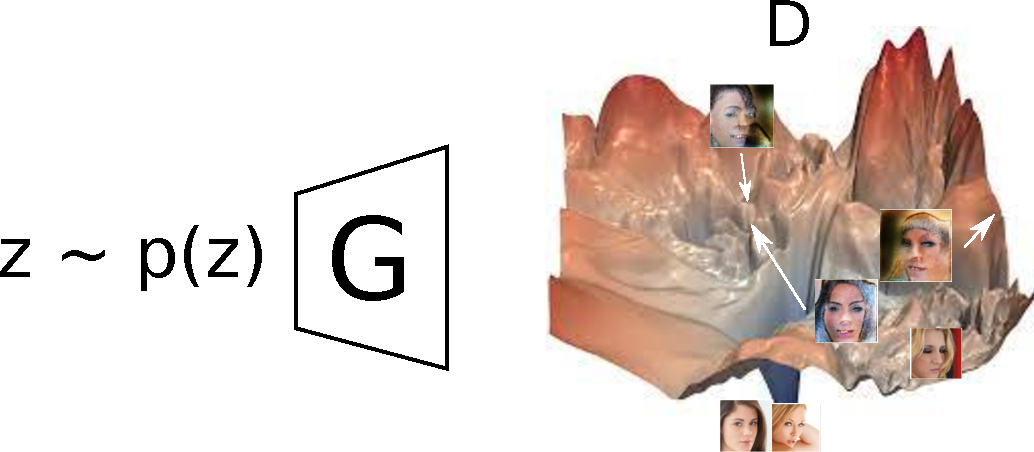
\includegraphics[scale=0.6]{60-files/gan-as-loss-bad.pdf}
    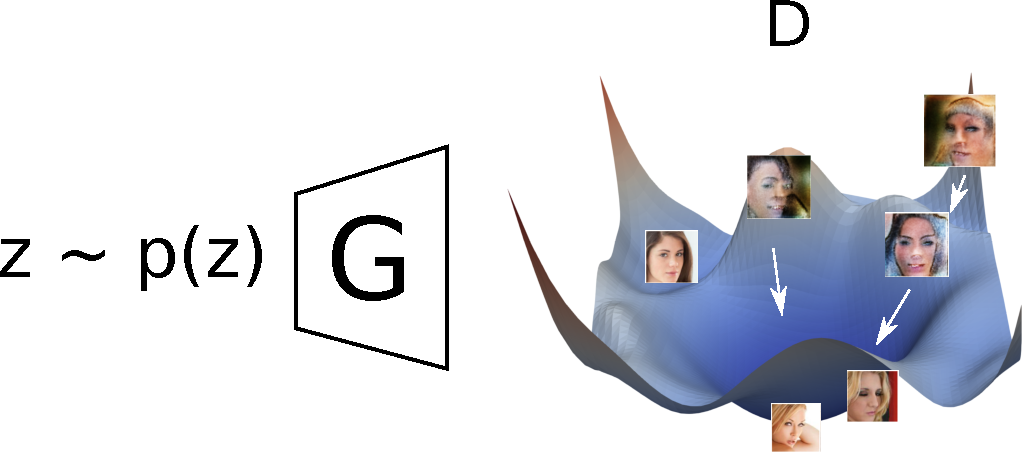
\includegraphics[scale=0.6]{60-files/gan-as-loss.pdf}
    \caption{Effect of regularizers. \textbf{Top}: $D$ is trained without a regularizer. The loss landscape might be noisy and hard to optimize against. There are strong peaks and valley because of the unregulated Lipschitzness. \textbf{Bottom}: $D$ is trained with R1 or \ac{WGAN-GP} regularizers, smoothing the surface around real data points or just controlling D's Lipschitzness. The gradients are more predictive of the correct optimization direction, the loss is easier to optimize against, the peaks and valley are smoother than the unregulated version. Note: these surfaces are just for illustrative purposes and are not visualizations of actual loss surfaces.}
    \label{fig:gan-lipschitz}
\end{figure}

In their analysis, \citet{R1}  exhibits that $R_\text{1-GP}$ brings rotational dynamics that slows down or totally hinders convergence. The system would oscillate around the convergence point as the gradients do not effectively point towards it but spiral around it. They present the $R_1$ regularizer that flattens the surface around real data points, effectively turning them into attractive points. Figure \ref{fig:gan-lipschitz} illustrates a regularized vs an unregularized loss landscape.

\begin{equation}
    R_1(D) = \IE_{x \sim \pdata} \nabla_x D(x)^2
\end{equation}

This strategy was successful enough to be used in and make the glory of StyleGAN \citep{stylegan}. Though, this regularizer does not enforce anything about D's Liptschitzness and diverges from the Wasserstein GAN framework.

\subsubsection{Beyond Wasserstein}

However as shown in \citet{aregansequal}, no loss for $D$ can ensure proper convergence. \citet{lipschitzgan} shows that any loss would work with a good Lipschitz regularization as those loss functions would be constrained in a linear regime anyway. This explains why \citet{R1}, despite not being rooted in \ac{WGAN}, shows better theoretical and empirical convergence than \ac{WGAN-GP}'s 1-GP regularizer. \citet{0-GP} pushes this idea further for greater generalization by flattening the path from real samples to fake samples.

\subsubsection{Image Synthesis}

Advances specific to image synthesis were mostly brought in the form of architectural refinements in $G$, starting from the Deep Convolutional GAN \citep{dcgan}, residual GANs introduced with SNGAN \citep{SNGAN}, progressively grown GANs \citep{progan}, or with multiscale noise inputs and adaptive scaling \citep{spade,stylegan,stylegan2} as seen in fast style transfer \citep{faststyletransfer}.

\section{Conditional Modeling}

Conditional generative models don't learn to replicate the full, unconditional $p(x)$ but instead learn to reproduce $p(x | y)$ with condition $y$, usually a class label or another data point. For instance, one might want to change pictures of satellites views into schematics for maps services. Or colorize edge sketches.

In most of those approaches, $x$ and $y$ are known, and the mapping is unknown. For this reason, they are often called "supervised" techniques since there is an input and a known output.

However \emph{generative modelling allows to model not a single output but a distribution of outputs}. There is more than one way to smile, and there are many possible pictures with class label "car". Common supervised techniques fail to acknowledge those situations.

This is the framework we are interested in for controlled data augmentation : we wish to generate random pictures for a given identity label. 

\subsection{Conditional GANs (cGANs)}

\subsubsection{cGANs}

Conditional GANS were first introduced by \citet{cgan}. They propose to concatenate the condition $y$ to the noise vector $z$ in $G$ and $y$ to the fake images $x_f$ and  real images $x_r$ in the Discriminator. That way, $D$ learns to discriminate whether $x$ and $y$ are in accordance and $G$ is taught to produce data points $x_f$ in accordance with $y$.

In this paper, $y$ is a one-hot class label encoding. They generate class conditioned MNIST and CIFAR samples.

\subsubsection{Pix2Pix}

\begin{figure}
    \centering
    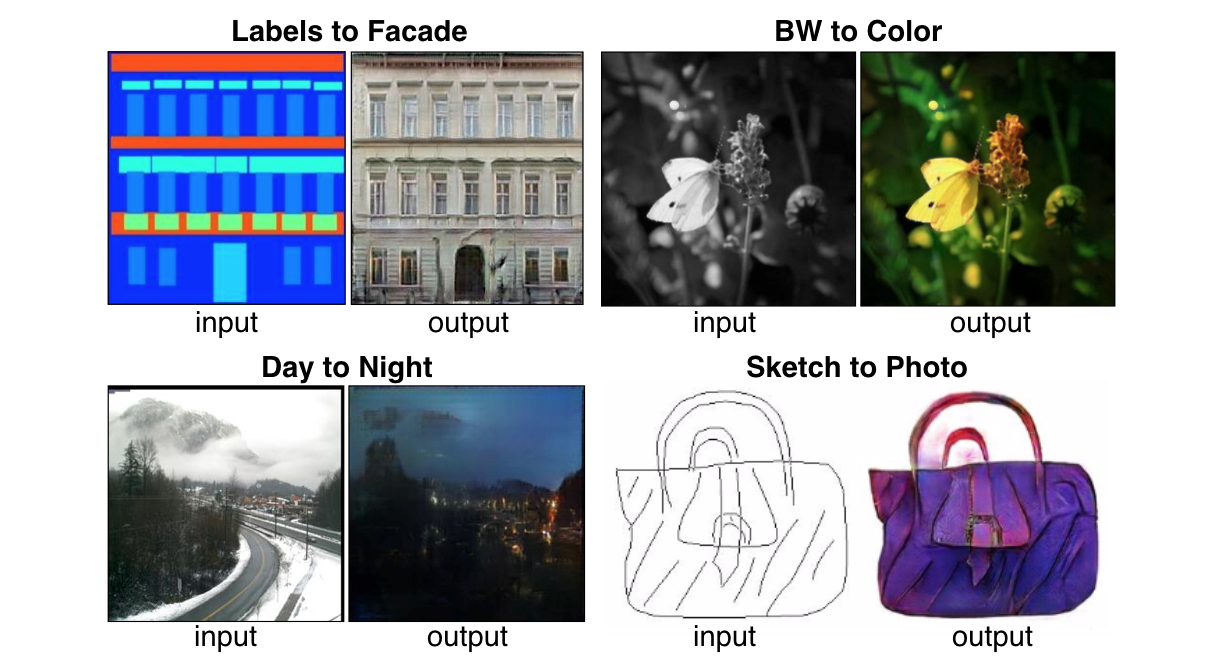
\includegraphics[width=\columnwidth]{60-files/pix2pix.png}
    \caption{Examples of image translation from the original pix2pix paper.}
    \label{fig:pix2pix}
\end{figure}

\citet{pix2pix} conditioned images based on images and was highly successful at supervised image translation, that is, \emph{transforming pictures from one domain to another}. Back then, gradient penalties were unknown and Lipschitzness was not a concern, thus Pix2pix and its evolution Pix2PixHD \citep{pix2pixhd} had to bake in several stabilization techniques like a supervised pixelwise loss and feature matching. Figure \ref{fig:pix2pix} shows examples from the original paper.

\subsubsection{BiGAN}

Unconditional GANs show that they have a semantic interpretation of their latent variable $z$. BiGAN \citep{bigan} proposes to jointly learn a generator $G: z \mapsto x$ and an encoder $F: x \mapsto z$ using a conditional discriminator $D$ that learns to discriminate $D(z, G(z))$ against $D(F(x), x)$. They prove that $D$ can be fooled only if $G = F^{-1}$. They then use $F$ as a feature extractor.

\subsection{Conditional VAEs (CVAE)}

\citep{cvae} introduced a CVAE, aiming to learn a conditional decoder $p(x|z,y)$. They replace the standard VAE encoder $q(z|x)$ with $q(z|x, y)$ and decoder $p(x|z)$ with $p(x|z,y)$. The conditioning variable $y$ can be changed at will to control the produced samples.

\section{Constrained Modeling}

Sometimes though, the pairs $(x, y)$ are unknown or the end goal is not suitable for conditional modeling. In those situations, it is possible to use constrained modeling, that is, generative modeling with additional constraints represented as additional loss terms. The generator must then compromise between matching the distribution matching loss enforced by the discriminator and satisfy the additional constraints losses. Sometimes, the constraints and distribution matching do not share a common minimum.

\subsection{InfoGAN}

One such example is the InfoGAN \citep{infogan} aiming to learn a controllable generator with disentangled input features. They learn a generator $G(z, c, f)$ with $z \sim p_Z(z)$ the latent variable distribution, $c \sim C$ with $C$ a user-chosen distribution of categorical random variables, and $f \sim F$ with $F$ a user-chosen distribution of continuous random variables. $G$ is trained against an unconditional discriminator $D(x)$ like in unconditional modeling, and another recognition network aiming to guess $c$ and $f$ from the generated sampled. $G$ and Q collaborate in order to maximize the mutual information $I(Q(c, f|G(z, c, f)); G(z, c, f))$. We aim for $G$ to learn to learn to use $c$ and $f$ as discoverable latent variables in the generative process, while enforcing the generated samples distribution $\pfake$ to be similar to $\pdata$.

$Q$ can then be used as a disentangled features extractor, or $G$ as a controllable generator.

\subsection{CycleGAN}

\begin{figure}
    \centering
    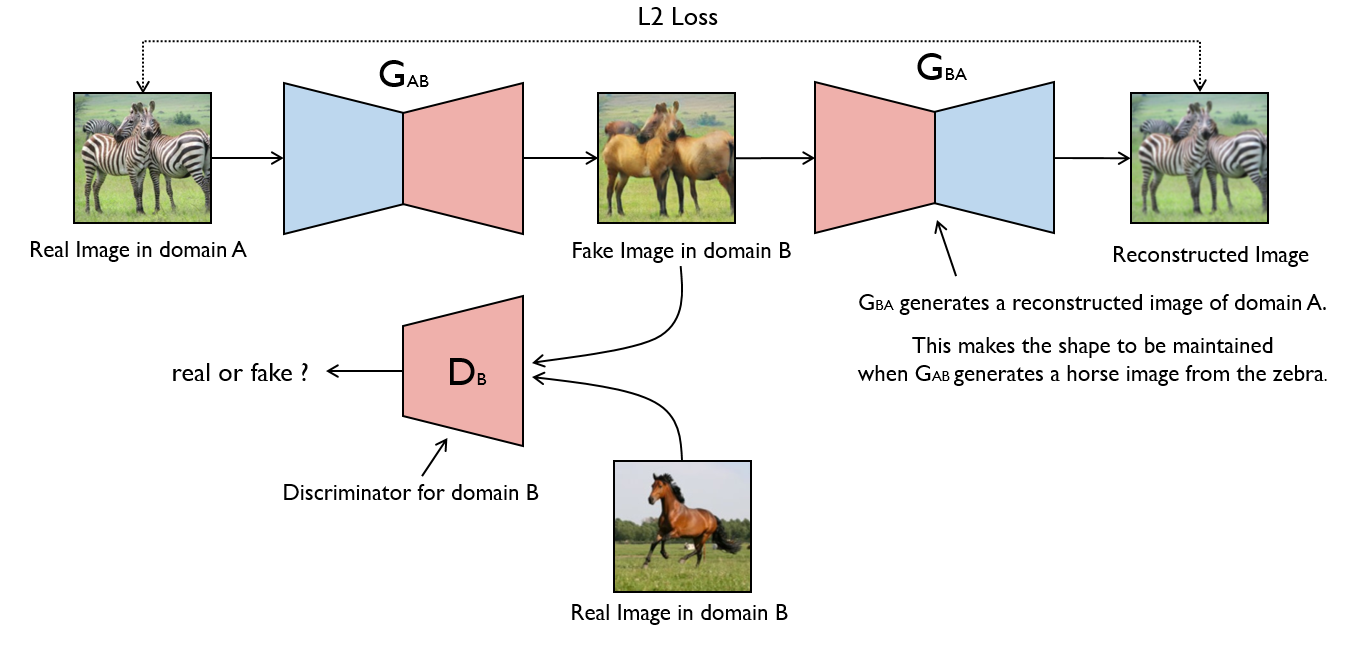
\includegraphics[width=\columnwidth]{60-files/cyclegan.png}
    \caption{The CycleGAN architecture. Image from \url{https://towardsdatascience.com/image-to-image-translation-using-cyclegan-model-d58cfff04755}}
    \label{fig:cyclegan}
\end{figure}

\citet{cyclegan} wanted to take Pix2Pix one step further and perform image translation \emph{in case pairs are not available}. We have real data points from real distribution $x_\text{a, real} \sim A$ and  real data points from real distribution $x_\text{b, real} \sim B$. We wish to learn a generator $G_{A \mapsto B}: z, x_\text{a,real} \mapsto x_\text{b, fake}$. They propose to learn two generators, $G_{A \mapsto B}$ and $G_{B \mapsto A}$, which respectively perform distribution matching against their own discriminator, respectively $D_B$ and $D_A$. This alone would ensure that both generators would produce realistic samples of their target distribution. However, we also want the output to bear some similarity with the input. This additional constraint is added as a cycle loss aiming for $x_a == G_{B \mapsto A}(G_{A \mapsto B}(x_a))$ and $x_b == G_{A \mapsto B}(G_{B \mapsto A}(x_b))$ and is is modeled with a L2 pixelwise similarity constraint. See Figure \ref{fig:cyclegan}.

While being a breakthrough, CycleGAN exhibits two major flaws. First, the L2 pixel-wise similarity constraint prevents the GAN from performing geometric heavy changes. Second, the cycle loss prevents any transformation that would loose information. For example, CycleGAN can't be used correctly for glasses removal as removing the glasses in a convincing way would make it impossible to recreate the exact same glasses to complete the cycle. In those situations, CycleGAN adds artifacts in order to be able to complete the cycle.

\subsection{Contrastive Unpaired Translation}

CUT \citep{cut} used contrastive learning to enforce the similarity constraint and improve on CycleGAN. They have a generator $G_{A \mapsto B}$, a discriminator $D_B$ that ensures realistic samples of $B$ are produced, and a matcher $M$. $M$ compares real and fake pairs of source image patches and output image patches with a contrastive loss, $G$ cooperates to ensure $M$ gets low loss.

This allows destructive transformations as there is no cycle loss, and allows shape transform as the constraint is not enforced on pixels but on deep features.

\section{Controlled Unconditional GANs}

Finally, while unconditional GANs are supposed to decode a random noise into a sample ($x=G(z)$), a growing set of work focus on deciphering the random noise space. It has been observed that the generators actually organizes the random noise input into semantically meaningful information \citep{bigan,bigbigan}.

\emph{These methods would enable reusing massive GANs that are expensive to train, such as StyleGAN2 or BigGAN, to fit different scenarios.}

Some work try to learn, a posteriori, a mapping from labels to latent subspaces, from few shots. This allows to create a controlled label-conditioned GAN from less annotated data than needed by a conditional GAN. \citet{interpretingz} learns latent directions from labels. \citet{ganspace} discovers disentangles directions from self-supervised learning.

Some other work focus on casting back real samples to the latent space, called \emph{GAN inversion}, by modeling $z=G^{-1}(x)$. They then transform the latent vector, and decode it back, in order to transform the original sample. Some optimize $z$ from a single sample, like \citet{inverting} while others like \citet{collaborativeembedding} learn encoders.

A fair amount of work in this framework tackle the inversion problem in order to make $G(G^{-1}(x))$ as close to $x$ as possible, and into identifying semantically meaningful and disentangled latent directions. Concretely, in the context of a face generation GAN, let $f_\text{smile}(z)$ be a function that maps a latent vector into its smiling face counterpart. The method is $G(f_\text{smile}(G^{-1}(x)))$, and the challenge lies into creating good algorithms to provide $G^{-1}$ and $f_\text{smile}$. Several transformation methods have been proposed. \citet{neuralphotoeditor} allows painting a target result by optimizing a pixel-wise L2 loss, \citet{interfacegan} identify latent directions with an auxiliary attribute classifier, \citet{pivotaltuning} first optimize $z$ then tune $G$ for better reconstruction with this $z$.

\section{Evaluation}

Evaluating GANs is difficult and must account for two key elements: image quality and distribution matching. In unconditional \ac{GAN}, the \ac{KID} \citep{kid}, \ac{FID} \citep{fid}, and slightly outdated Inception Score (IS) \citep{inceptionscore} are used to evaluate both elements at once. Those can also be evaluated separately with metrics such as the  Precision / Recall developed by \citet{precisionrecall}. Unfortunately it is quite unclear as of today how to evaluate a conditional \acp{GAN}, especially in the unpaired setting.

\subsection{FID}

The Fréchet Incepton Distance gained a lot of traction to evaluate image GANs. It works by fitting a multivariate normal distribution on the output vectors of an Inception-V3, encoding the real and generated images, and computing the Fréchet distance \citep{frechet} between both. For two gaussian $X$ and $Y$, the Fréchet distance is expressed as
\begin{equation*}
    F(X,Y) = \|\mathbf{\mu}_X - \mathbf{\mu}_Y\|^2 + tr\left(\mathbf{\Sigma}_X + \mathbf{\Sigma}_Y - 2\sqrt{\mathbf{\Sigma}_X\mathbf{\Sigma}_Y}\right)
\end{equation*}
where $\mathbf{\mu}$ and $\mathbf{\Sigma}$ are the mean and co-variance of the subscripted Gaussian.
This captures both the realism of the generated images and the coverage of the modes and variance of the real distribution.

While the FID is widely used, it has some drawbacks. It is biased and as such limited for small dataset, is not easily interpretable, and is meant for evaluation of unconditional GANs.

\subsection{\acs{KID}}

The Kernel Inception Distance serves the same purpose as the \ac{FID} but has a different mathematical expression that makes it unbiased. It uses the polynomial kernel $k(\mathbf{x},\mathbf{y}) = \left(\frac{1}{d}\mathbf{x}^T\mathbf{y} + 1\right)^3$, where $d$ is the number of dimension of $\mathbf{x}$ and $\mathbf{y}$, which are the Inception representations of the images. Not having to compute this metric on 50k samples as is traditionally done for the \ac{FID} makes it more suitable for smaller datasets. It has been recently used in pair with the \ac{FID} for comparing methods.

\subsection{Precision / Recall}

\begin{figure}[!h]
    \centering
    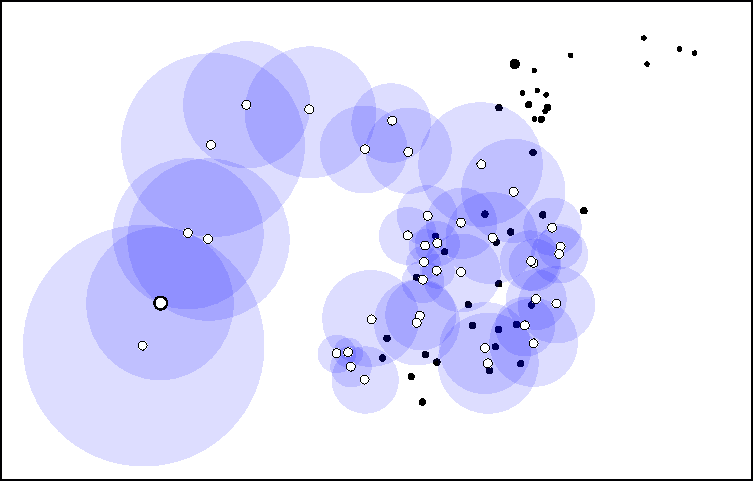
\includegraphics{60-files/precision-gan.pdf}
    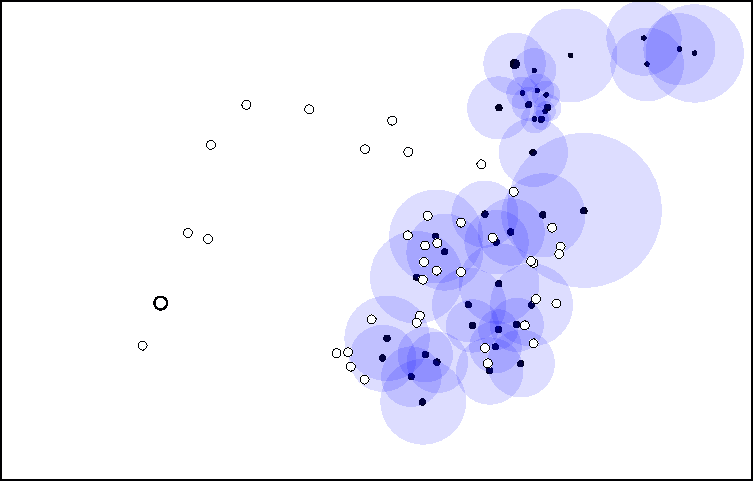
\includegraphics{60-files/recall-gan.pdf}
    \caption{Precision/Recall estimation: white dots are 2D representations of generated samples and black dots are real samples representations. Top figure shows the fake manifold estimation (in blue), the ratio of black dots inside the manifold shows the recall, ie, the ratio of the real dataset covered by the generator. Below, we show the manifold of the real dataset. The ratio of white dots inside the blue zone is the precision, ie, the ratio of generated samples that look like real samples. For those visualization we set $k=2$}
    \label{fig:precision-recall}
\end{figure}


Perhaps more relevant to our work is the precision / recall metrics developed by \cite{precisionrecall}, that separate the evaluation of image quality and target distribution coverage.

Both those metrics use a density estimation technique to approximate the manifold of the real images and generated images. The ratio of generated images included in the real manifold is called precision and correlates with image quality. The ratio of real images included in the fake manifold is the recall and expresses how much of the real data has coverage in the fake manifold.

In order to estimate a manifold, we draw a sphere from each sample to its $k$-th nearest neighbor. A point inside one of those spheres is considered inside the manifold. For image data, we don't use the pixel values but deep features from a VGG or inception network and usually set $k=2$ or $k=3$.

Precision reflects the image quality without accounting for the distribution difference in the conditional setting. Recall measures how much of the training data is covered by the generated distribution.

All those metrics are implemented in Torchélie.

\section{\emph{\arr Contribution}: Expiration date for VQ codebooks}

Some works \cite{robustvq} observed that VQ-VAEs fail to manipulate efficiently the entirety of the quantized vectors available, some remaining unoptimized for the entirety of the training procedure. Earlier works explored different initialization strategies or periodic resampling of quantized vectors by k-means. We propose a simpler and lightweight algorithm that even allows choosing the perplexity of the quantized vectors usage.

\subsection{Principles}

\begin{figure}[ht]
    \centering
    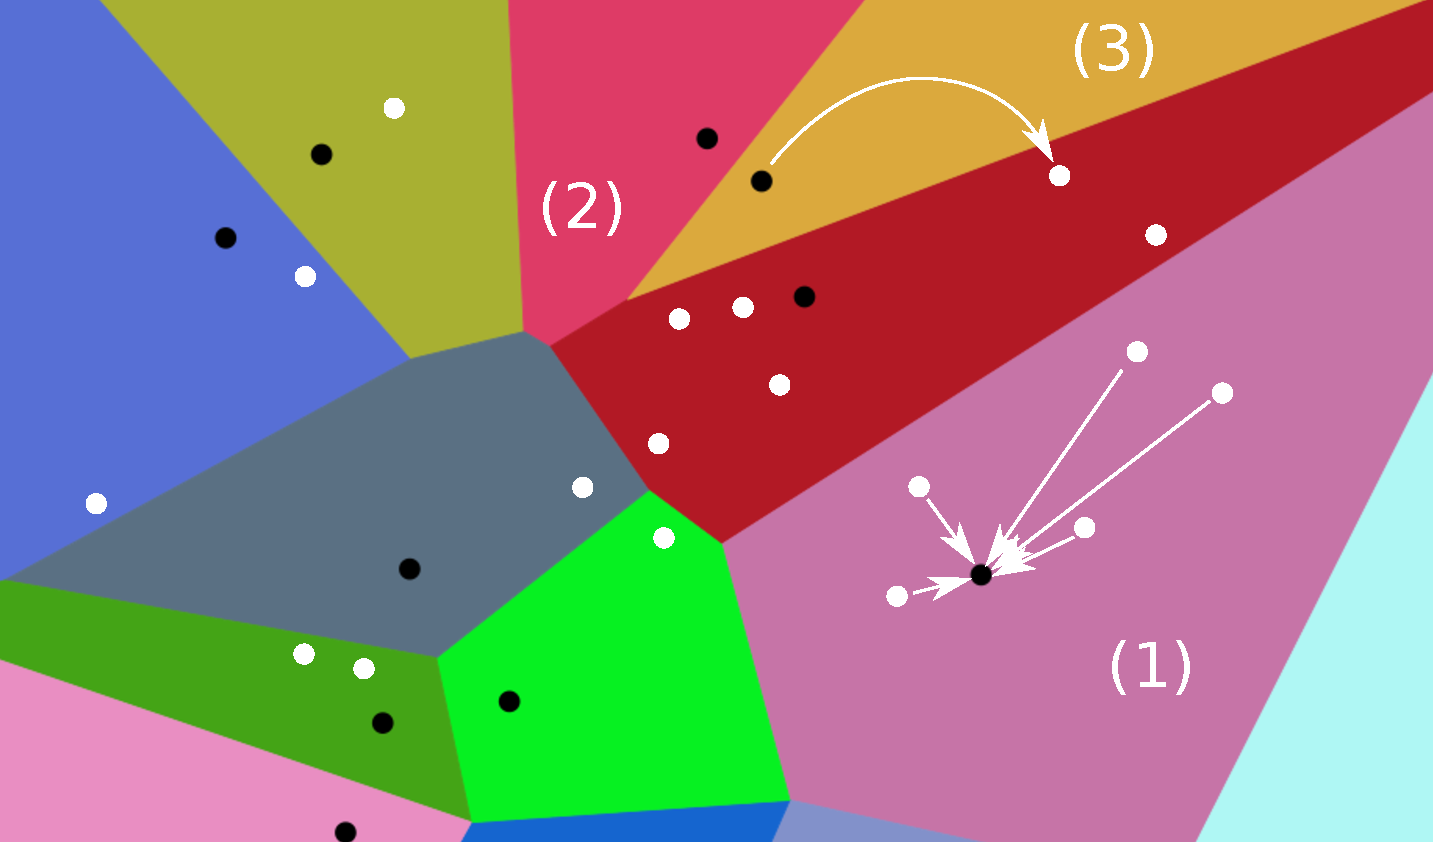
\includegraphics[scale=0.5]{60-files/vq.pdf}
    \caption{A VQ layer. Black points are codebooks prototypes. They divide the space into Voronoi cells. White points are input vectors, quantized to the prototype of the Voronoi cell they fall in. (1) shows the commitment loss as white arrows, bringing the input vectors closer to the prototype they have been assigned to. The prototype in cell (2) is not used in this iteration, its unused age is incremented. When, like in cell (3), that prototype has not been used for too long (more iterations than $\texttt{max\_age}$), it is resampled to a random input vector and its age is reset to 0. }
    \label{fig:vq-resample}
\end{figure}

It became quickly clear that the quantized vectors in the codebook are updated only via weight decay or receive gradients only if input vectors are quantized to them. If initialized improperly, a significant part of the codebook might not be ever used and just lost. Some codes might be lost as well during training if the updates of the codebook and input vectors get out of sync.

To overcome this issue and ensure a full usage of the codebook, and thus of the available bandwidth, we chose to resample every so often the codebook based on k-means centroids of the previous input vectors. This approach is laid out in \citet{robustvq}. Others have proposed continuous relaxation \citep{continuousvq} or soft assignments \citep{softvq}.

\begin{figure}
\begin{lstlisting}[language=Python, caption=VQ with expiration (pseudo python),label={code:vq}]
class VQ:
    """
    Quantization layer from *Neural Discrete Representation Learning*
    Args:
        latent_dim (int): number of features along which to quantize
        num_tokens (int): number of tokens in the codebook
        return_indices (bool): whether to return the indices of the quantized
            code points
    """
    def __init__(self, latent_dim: int, num_tokens: int, max_age: int):
        self.embedding = Array(num_tokens, latent_dim).gaussian_init()
        self.age = Array(num_tokens).fill(max_age)
        self.max_age = max_age

    def forward(self, x: torch.Tensor):
        if self.training:
            for i in range(len(self.age)):
                if self.age[i] => self.max_age:
                    self.embedding[i] = random.choice(x)
                    self.age[i] = 0

        codes, indices = quantize(x, self.embedding)

        if self.training:
            for i in range(len(self.age)):
                self.age[i] += 1

            for i in indices:
                self.age[i] = 0

        return codes
\end{lstlisting}
\end{figure}

Instead, we propose a simpler algorithm. Prototypes that have not been used for more than $\texttt{max\_age}$ iterations are resampled to a random vector of the current batch. This allows to directly set a lower bound on the entropy of the assignments: a lower expiration timer will push towards uniform assignments  while a higher timer would allow for stronger unbalance and preferences.

Our approach is implemented in Torchélie and supports distributed training. Figure \ref{fig:vq-resample} illustrates various elements of the VQ layer, Listing \ref{code:vq} is a pseudo-python simple implementation.

\subsection{Experiments}

\subsubsection{Metrics.}

I evaluate the proposed algorithm under various codebook sizes, in both training and testing. Perplexity is used to estimate the codebook usage, as well as the age of the different codes. Finally, the influence on the test loss is considered as well; the test set contains 512 pictures.

The experiments are ran on an autoencoding task. We encode 128x128 Imagenette \citep{imagenette} into a spatial map of 8x8 codes. The number of available codes varies through experiments. 

\subsubsection{Training and age.}

\begin{figure}
    \centering
    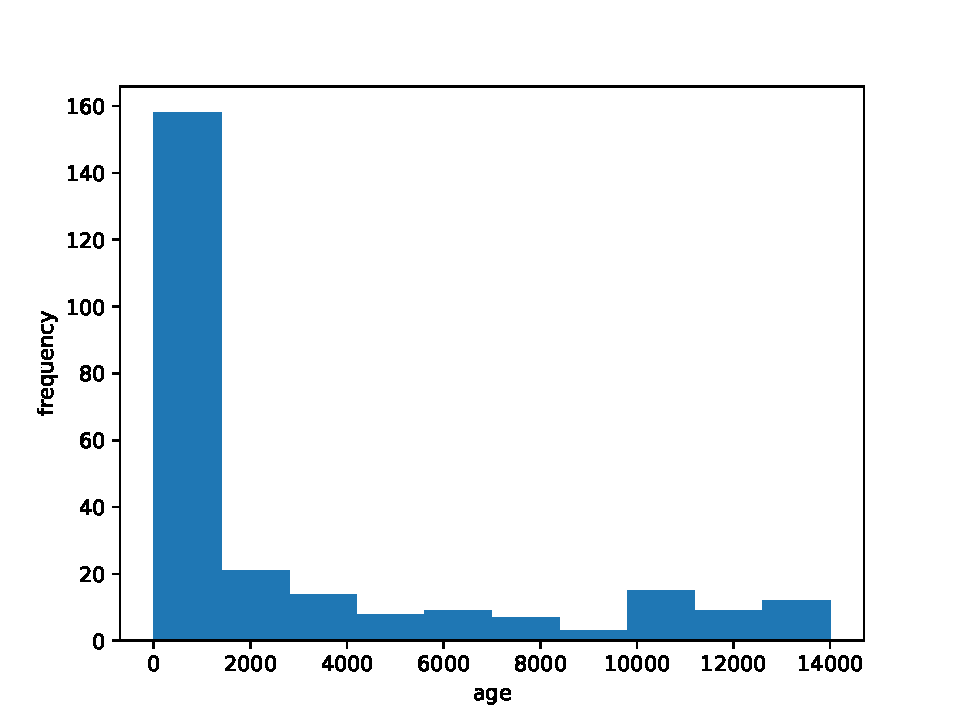
\includegraphics[width=0.45\columnwidth]{60-files/age.pdf}
    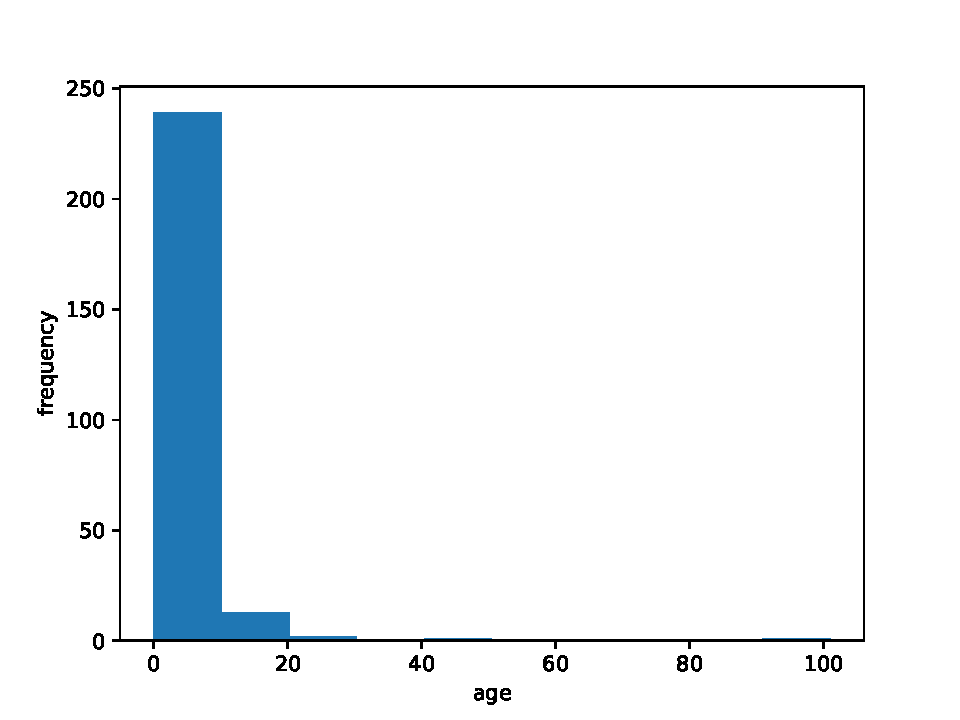
\includegraphics[width=0.45\columnwidth]{60-files/age-aging.pdf}
    \caption{Age (time since last use) of each VQ layer codepoint. \emph{left:} Without the expiration process, the optimization is harder and the net fails to use the codebook to optimize the loss. A lot of the codes remained unused for at least 2k iterations, presumably dead. \emph{right:} Expiring and resampling code allows for exhaustive use of the codebooks and controllable entropy. Even if the maximum age is set to 250 iterations, the codebook has a much lower age on average.}
    \label{fig:agingvq-age}
\end{figure}

Figure \ref{fig:agingvq-age} shows the age of the code points after 20k training iterations (50 epochs). As expected, with expiration, the codes have all been recently utilized with a median age of 0 and a mean age of 4. Even the oldest code is 150, less than the expiration period (250 iterations). Without the expiration strategy, and despite the Batch Normalization preceding it \citep{robustvq}, most code points have not been used at all, showing an age of 20k. In this situation, the bottleneck is actually much stronger than expected, making it hard to design and reason about its size.

\begin{figure}
    \centering
    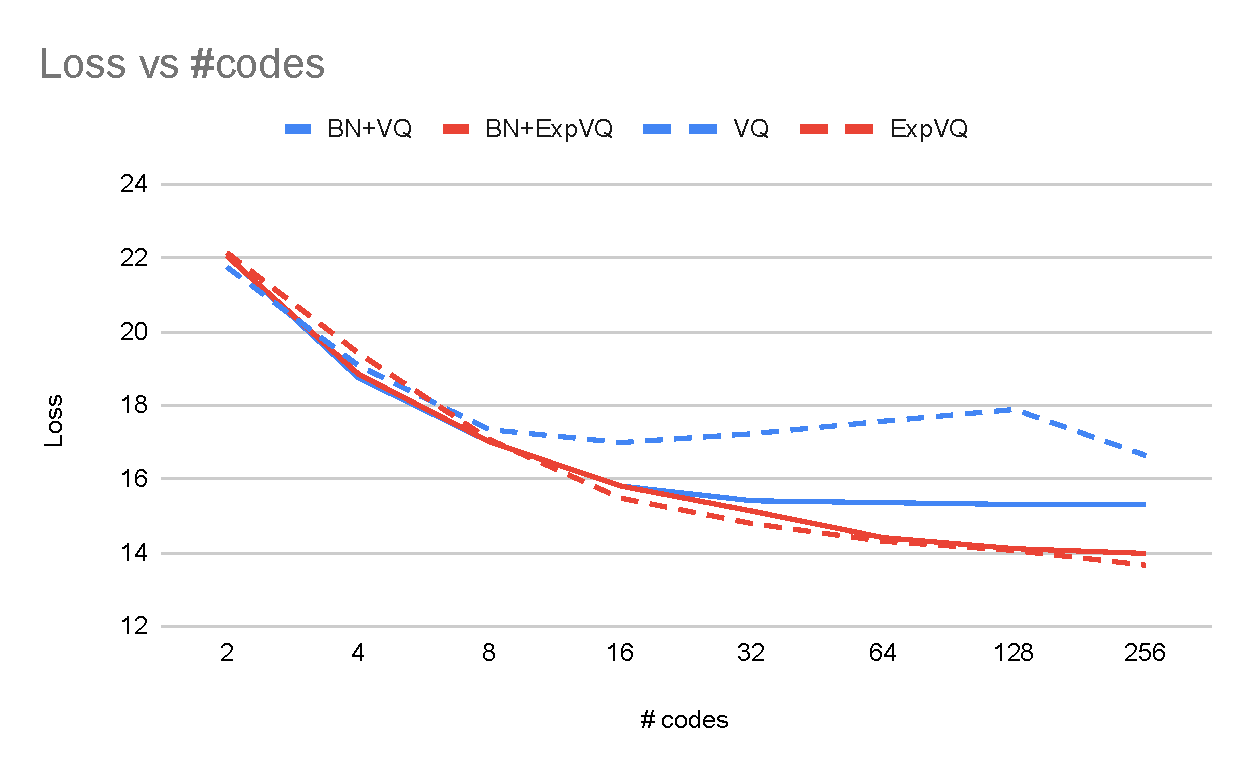
\includegraphics[width=0.45\columnwidth]{60-files/chartloss.pdf}
    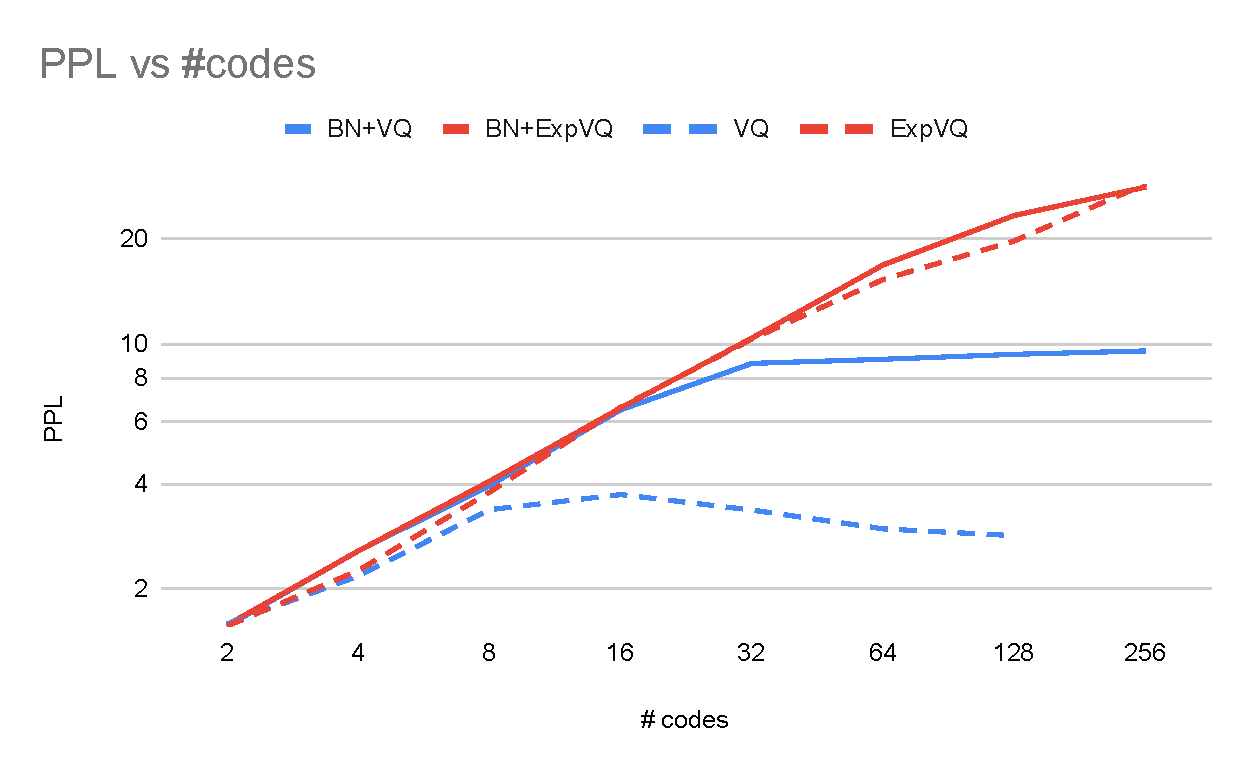
\includegraphics[width=0.45\columnwidth]{60-files/chartppl.pdf}
    \caption{Experiment comparing test loss (left) and codebook usage PPL (right) with a ReLU layer before quantization. The standard initialization is not robust to this situation.}
    \label{fig:agingvq-training-nobn}
\end{figure}

Figure \ref{fig:agingvq-training-nobn} displays the loss and PPL with a ReLU instead of a batch normalization layer before the quantization. Our expiration process allows to quickly replace the codes initialized in the negative area. This allows a greater robustness to initialization and architecture, being more error tolerant as well.

\subsubsection{One codebook of size N}

In the next series of experiments, the bottleneck is reduced to a single codebook of N code points, varying N. The quantized vector has 8 dimensions. We budget each experiment with the number of iterations needed for the expiration strategy to converge.

The Figure \ref{fig:agingvq-32} shows the test loss and PPL for increasing codebook size.

\begin{figure}
    \centering
    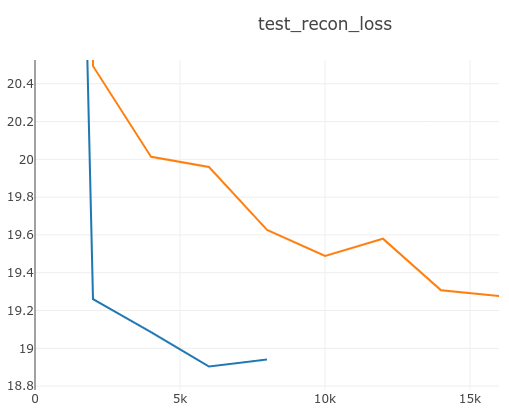
\includegraphics[width=0.45\columnwidth]{60-files/loss-32.png}
    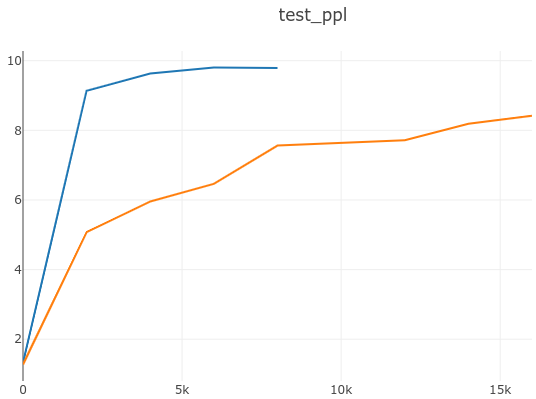
\includegraphics[width=0.45\columnwidth]{60-files/ppl-32.png}
    \caption{Experiment comparing test loss (left) and codebook usage PPL (right) for a codebook of 32 code points.}
    \label{fig:agingvq-32}
\end{figure}

\paragraph{For small codebooks.}
A deeper experiment for 32 code points shows in Figure \ref{fig:agingvq-32} that, with a relatively small codebook, more training manages to gradually recover full usage of the codebook, although much more slowly than its expiration counterpart. In fact, training twice as long does not suffice to reach the the same loss.

\paragraph{For big codebooks.}
Taking this experiment to more code points yields a different result: most of the codes remain unused, and, contrarily to the previous results, are not "recovered" thanks to more training iterations. In this situation, the expiration strategy becomes necessary in order to control the effective bottleneck size and not to waste unused parameters.

\paragraph{Follow up.}
I hypothesize that those results are amplified for dimensions greater than 8 because of the curse of dimensionality, but this is still to be verified experimentally.

\subsection{Conclusion}

We proposed a simple and lightweight algorithm that allows setting a lower bound on the entropy of the codebook usage in VQ-VAEs. Experimental evidence suggest that this strategy yields improvements over the baselines that grows with the size of the codebook. Our results show that our proposed algorithm show no notable inferiority scenario, and can be used as a default safely. 

\section{\emph{\arr Contribution}: A Latent Variable Model for facial pose generation}

\begin{figure}[ht]
    \centering
    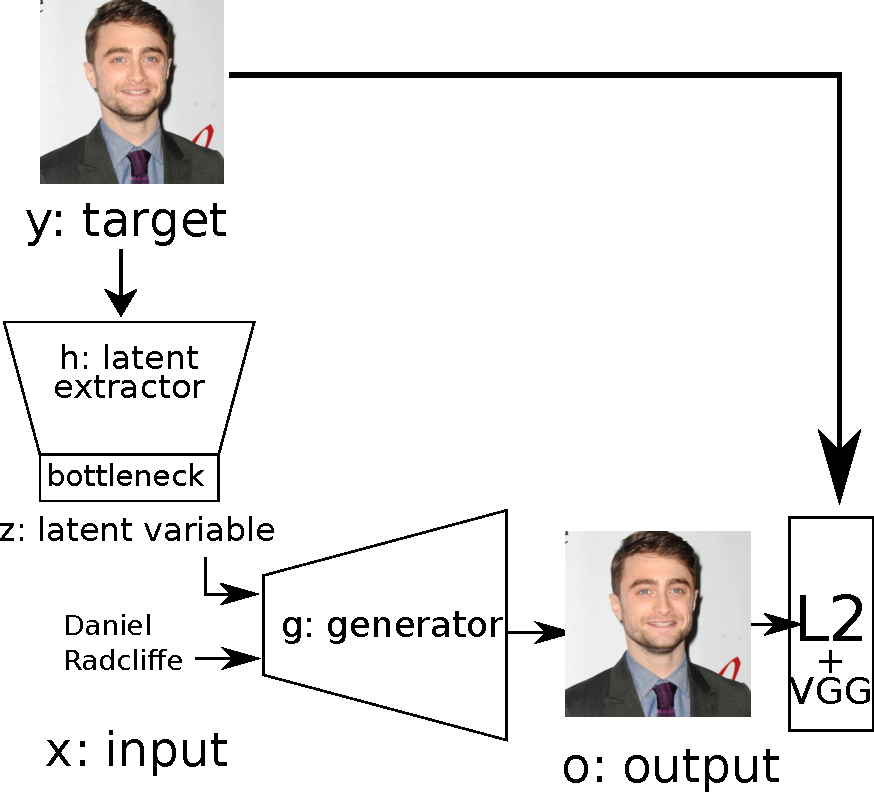
\includegraphics[scale=0.75]{60-files/latent-facegen.pdf}
    \caption{Our proposed controllable face generator. A target face is encoded to a latent, decoded back with the identity label to the original picture. An information bottleneck in the encoder discourages the latent variable to contain any information about the person's identity, thus not leaking any identity specific geometry and encoding parameters not recoverable from the identity alone: lighting, pose, makeup, etc. At inference time, one can use any latent from any sample or sample a latent from a prior distribution to reenact anyone's face.}
    \label{fig:latent-facegen}
\end{figure}

\subsection{Problem setting}

We saw in the latent variable model (Section \ref{sec:lvm}) a way to disentangle known factors from the rest in a generative process. In the situation we are interested in, face generation with controllable identity, we wish to learn a generative process able to disentangle facial geometry, specific to a given identity, from other factors such as pose, pixels location in picture, lighting, saturation. Some other factors are more ambiguous such as makeup, hair style, or age that may or may not change according to identity and can sometimes help to recognize someone.


\subsection{Methods}

\subsubsection{Architecture}

The system we prorpose is a latent variable model in the form of an encoder-bottleneck that extracts latent variables from a picture, and sends them to the decoder along with an identity embedding. We aim to reconstruct the input image under a L2 pixel-wise loss and a VGG loss (also called Perceptual loss). The VGG loss is the L2 difference of deep features of pretrained VGG network.

We choose simple convolutional encoders and decoders following a VGG style for both the encoder and decoder. The encoder uses quantification bottleneck as we have seen it produces crispier pictures.

Figure \ref{fig:latent-facegen} shows our proposed approach.

We emphasize the importance of image quality since the produced samples are to be used as training data.

\subsubsection{Training}

We train the model on aligned faces from Hexaglobe with RAdamW. The algorithm is implemented with Torchélie.

At inference time, we reuse latent variables from the training set but randomly swap identity vectors. Not only is this simple but also aligns with our goal of performing face swap. We could have trained an autoregressive model on the latent variables of the training set to be able to generate the latents themselves as well but generating new poses is not an objective of this work. Moreover, the training set is already large enough to propose a large diversity of latent variables. We evaluate our system under face swap quality and image quality.

\begin{enumerate}
    \item While not ideal, we score the quality of the face swap features by the ability of a face classifier to recover the new sampled identity.
    \item We compute the \ac{KID} \citep{kid} as our image quality metrics.
    % FIXME KID / Precision => pas de métrique de distribution matching (irrelevant)
\end{enumerate}



\subsection{Negative results}

\begin{itemize}
    \item We tried training the model with a Gaussian prior information bottleneck. The image quality was terrible (blurry), which is unsurprising from a standard \ac{VAE} approach. Moreover, the manifold of the latent variations was too complex to fill the whole Gaussian volume, resulting into many "holes" in the prior spaces. Sampling latents from the prior lead to results only slightly looking like faces, far worse than reusing extracted latents.
    
    \item We found the L2 pixel loss not sufficient and too harsh to generate meaningful images. This loss considers that all pixels are equal in the image, which is not true. Some pixels of the face, like face contours, bear more semantics than the others, like background pixels. A VGG loss captures this pixel importance and emphasize the importance of those pixel structures, while relaxing the need to reconstruct the target picture in a pixel-perfect fashion. The VGG loss compares image semantics rather than pixel intensities.
\end{itemize}

\subsection{Results}

After training our model, our face classifier recognizes the target identity 92\% of the time, showing that our model is successfully disentangling identity latents and pose latents. We reach a KID of 0.044. The generated images are somehow "too clean" and the background are not captured, showing a washed out "average background color" without any pattern. This is due to the L2 loss that encourages to produce an average (in this case, blurry) response when patterns fail to be captured. 

The results from our classification metric have to be discussed. This metric kind of contradicts itself: an excessively low result would indicate that the swapping fails, but a very high result would signal that our classifier perfectly recognizes the swapped identities. This would sound like a good thing, but it would actually show that the proposed data augmentation is useless. Indeed, this would indicate that our face classifier perfectly disentangles pose and face features, without learning shortcuts or overfitting on spurious elements. Whether or not the score of 92\% is an indication of the latter can only be known by computing the actual impact as a data augmentation, which is still to be done.

\begin{figure}[ht]
    \centering
    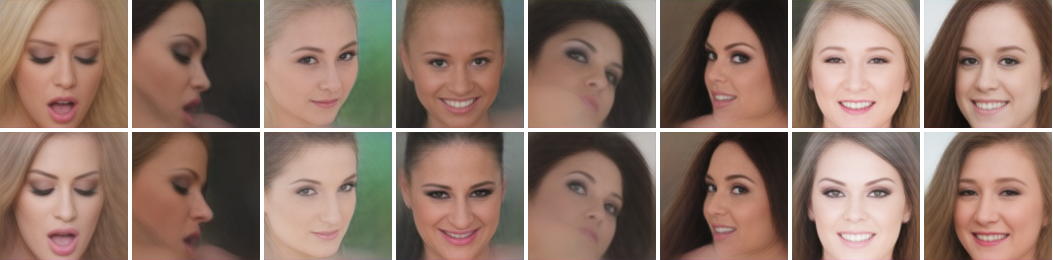
\includegraphics[scale=1.5]{60-files/resampled-1.png}
    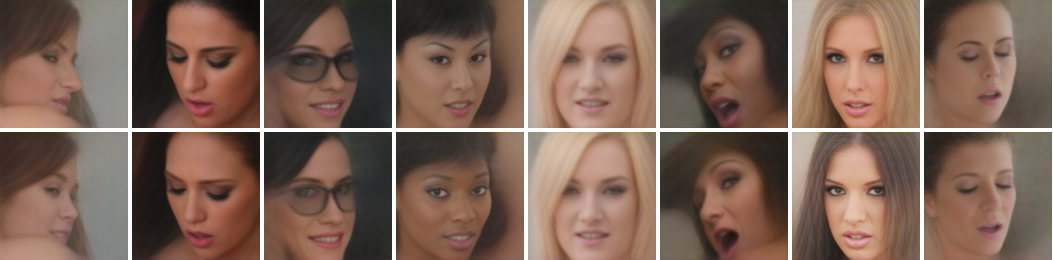
\includegraphics[scale=1.5]{60-files/resampled-2.png}
    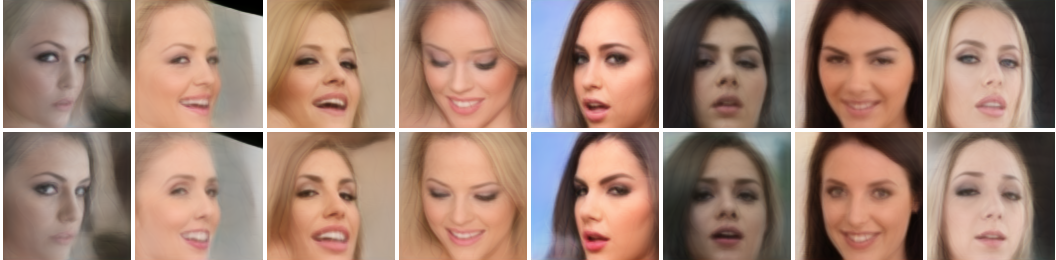
\includegraphics[scale=1.5]{60-files/resampled-3.png}
    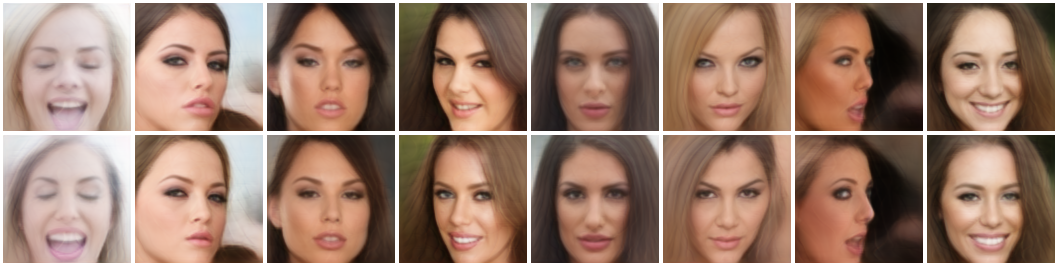
\includegraphics[scale=1.5]{60-files/resampled-4.png}
    \caption{Four batches of not curated samples. Rows 1, 3, 5, 7 are reconstructed samples. Identity is randomly swapped in rows 2, 4, 6, 8 but latent vector is kept untouched.}
    \label{fig:vqvae-facegen-samples}
\end{figure}

Figure \ref{fig:vqvae-facegen-samples} presents some resulting samples. The image quality is, as expected from a VQ-VAE, fairly good. Notice how the image from each couple of rows look identical but, upon closer inspection, actually display different identity-specific facial features (hair color, nose size, skin tone, eyes shape, etc).